\documentclass[tikz]{standalone}
\usepackage{amsmath}
\usepackage[T1]{fontenc}
\usepackage[utf8]{inputenc}


\usetikzlibrary{arrows,%
                shapes,%
                matrix,%
                decorations.pathmorphing,%
                backgrounds,%
                positioning,%
                fit,%
                petri}

%\usetikzlibrary{external}
%\tikzexternalize[prefix=tikz/]
\usepackage{mathpazo}

\begin{document}

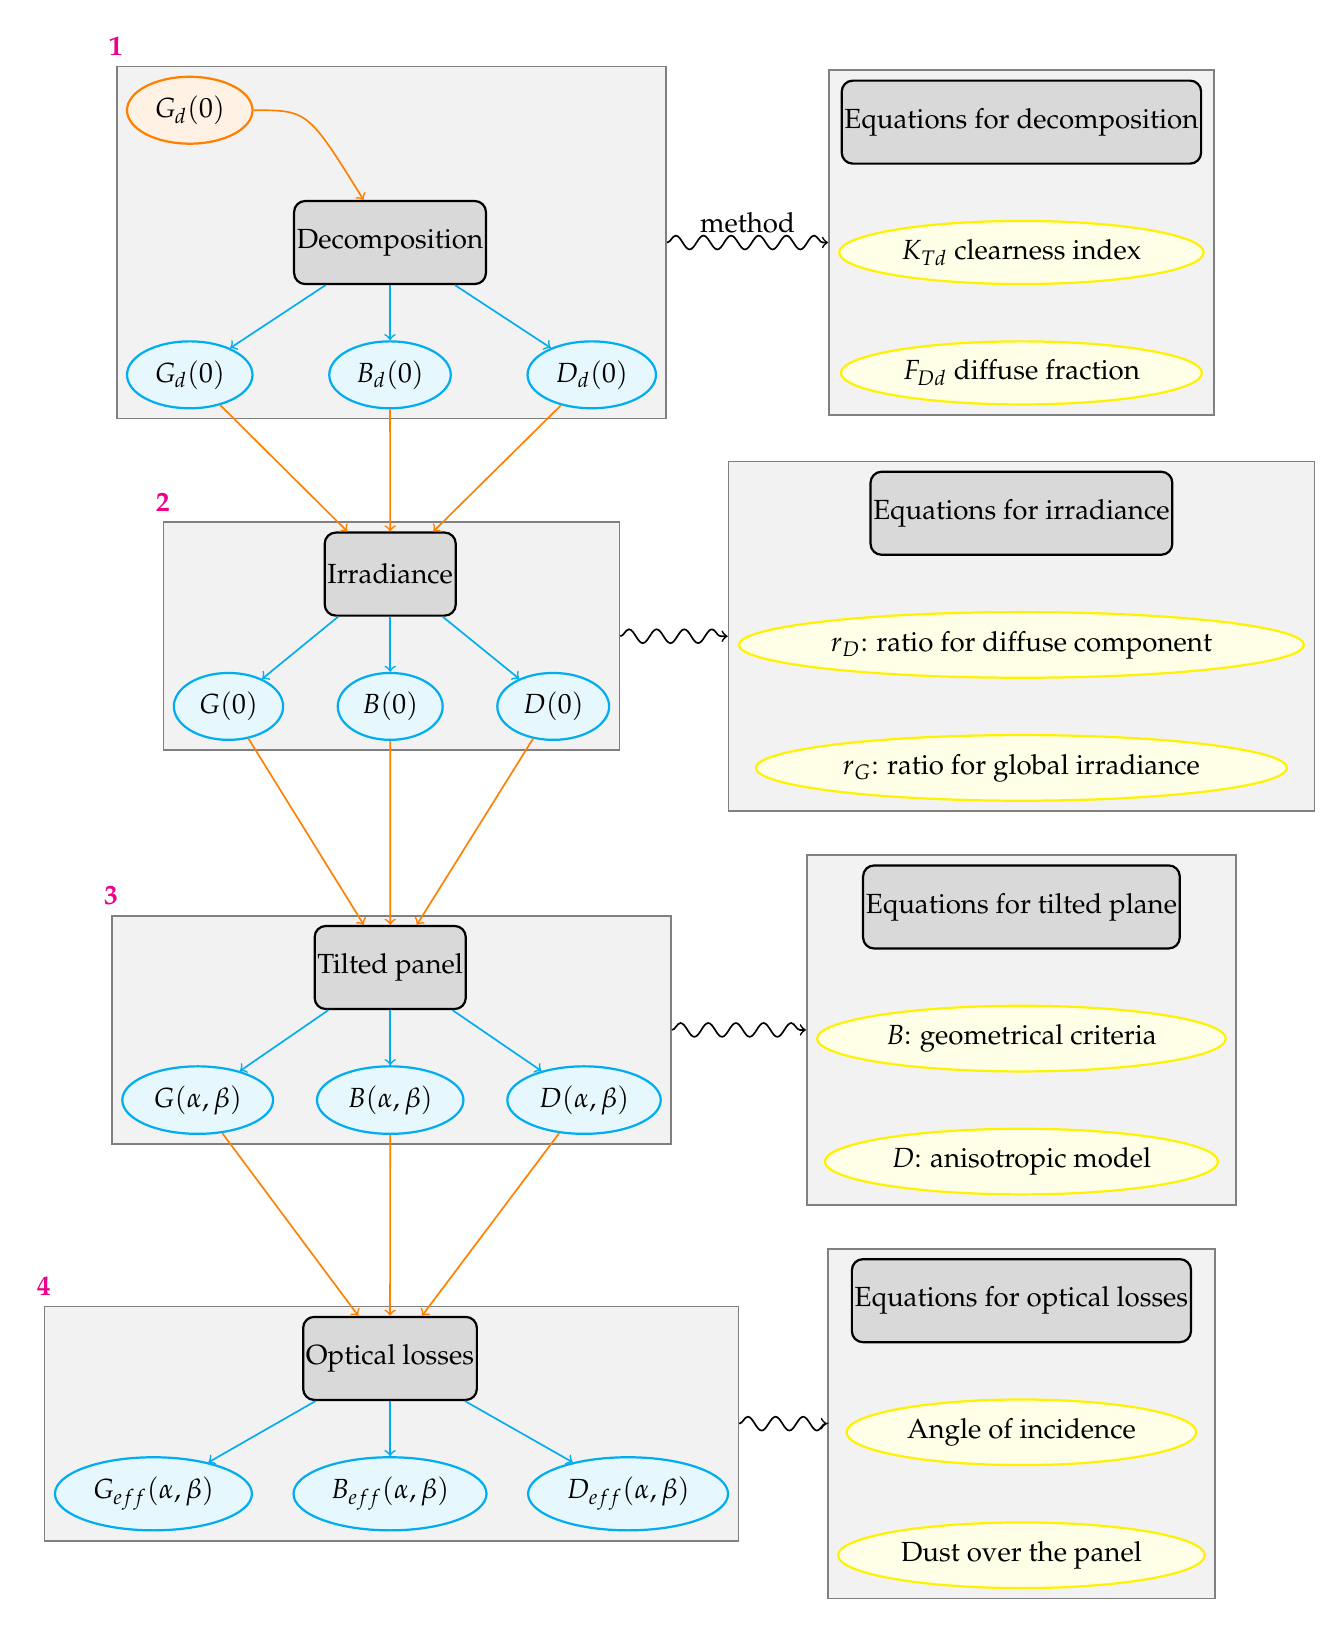
\begin{tikzpicture}[auto,
operation/.style={rectangle, rounded corners, draw=black, thick, fill=gray!30,
minimum height=3em, align=flush center, inner sep=1pt},
%
simple/.style={draw=black, circle, fill=gray!30},
%
source/.style ={draw=orange, thick, ellipse, fill=orange!10,
minimum height=2em},
%
result/.style ={draw=cyan, thick, ellipse, fill=cyan!10,
  minimum height=2em},
%
method/.style={draw=yellow, thick, ellipse, fill=yellow!10,
minimum height=2em}]
 
\tikzset{every path/.style={line width=.6pt}}

\begin{scope}
  \matrix[matrix of nodes, fill=gray!10, draw=black!50, column sep=5mm, row sep=7mm, minimum width=7mm] (disagreg){
        \node  [source] (GHI) {$G_{d}(0)$}; &
        \node  {}; &
        \node  {}; \\
        %%%%%%%%%%%%%%%%%%%%%%%%%%%%%%%%%%
        \node {}; &
        \node [operation] (decomposition){Decomposition}; &
        \node {}; \\
        %%%%%%%%%%%%%%%%%%%%%%%%%%%%%%%%%%
        \node [result] (G0d) {$G_d(0)$}; &
        \node [result] (B0d) {$B_d(0)$}; &
        \node [result] (D0d) {$D_d(0)$}; \\
};
\end{scope}
 
\begin{scope}[yshift=-5cm]
\matrix[matrix of nodes, fill=gray!10, draw=black!50, column sep=5mm, row sep=7mm, minimum width=7mm] (irradiance){
        %\node  [source] (G02) {$G(0)$}; &
        %\node  [source] (B02) {$B(0)$}; &
        %\node  [source] (D02) {$D(0)$};\\
        %%%%%%%%%%%%%%%%%%%%%%%%%%%%%%%%%%                                                                                   
        \node {}; &
        \node [operation] (irradiancia){Irradiance}; &
        \node {}; \\
        %%%%%%%%%%%%%%%%%%%%%%%%%%%%%%%%%%                                                                                   
        \node [result] (G0) {$G(0)$}; &
        \node [result] (B0) {$B(0)$}; &
        \node [result] (D0) {$D(0)$}; \\
};
\end{scope}


\begin{scope}[yshift=-10cm]
\matrix[matrix of nodes, fill=gray!10, draw=black!50, column sep=5mm, row sep=7mm, minimum width=7mm] (tiltedpanel){
        %\node  [source] (G02) {$G(0)$}; &
        %\node  [source] (B02) {$B(0)$}; &
        %\node  [source] (D02) {$D(0)$};\\
        %%%%%%%%%%%%%%%%%%%%%%%%%%%%%%%%%%                                                                                
        \node {}; &
        \node [operation] (plano inclinado){Tilted panel}; &
        \node {}; \\
        %%%%%%%%%%%%%%%%%%%%%%%%%%%%%%%%%%                                                                                 
        \node [result] (G) {$G(\alpha,\beta)$}; &
        \node [result] (B) {$B(\alpha,\beta)$}; &
        \node [result] (D) {$D(\alpha,\beta)$}; \\
};
\end{scope}

\begin{scope}[yshift=-15cm]
\matrix[matrix of nodes, fill=gray!10, draw=black!50, column sep=5mm, row sep=7mm, minimum width=7mm] (optical){
        %\node  [source] (G02) {$G(0)$}; &
        %\node  [source] (B02) {$B(0)$}; &
        %\node  [source] (D02) {$D(0)$};\\
        %%%%%%%%%%%%%%%%%%%%%%%%%%%%%%%%%%                                                                                
        \node {}; &
        \node [operation] (Optical losses){Optical losses}; &
        \node {}; \\
        %%%%%%%%%%%%%%%%%%%%%%%%%%%%%%%%%%                                                                                 
        \node [result] (Gef) {$G_{eff}(\alpha,\beta)$}; &
        \node [result] (Bef) {$B_{eff}(\alpha,\beta)$}; &
        \node [result] (Def) {$D_{eff}(\alpha,\beta)$}; \\
};
\end{scope}

\begin{scope}
  \draw[->, orange](GHI) .. controls ++(0:1.5) .. (decomposition);
  %%%%%%%%%%%%%%%%%%%%%%%%%%%%%%%%%%%%%
  \draw[->, cyan](decomposition) -- (G0d);
  \draw[->, cyan](decomposition) -- (B0d);
  \draw[->, cyan](decomposition) -- (D0d);
  %%%%%%%%%%%%%%%%%%%%%%%%%%%%%%%%%%%%
  \draw[->, orange](G0d) -- (irradiancia);
  \draw[->, orange](B0d) -- (irradiancia);
  \draw[->, orange](D0d) -- (irradiancia);
  %%%%%%%%%%%%%%%%%%%%%%%%%%%%%%%%%%%%
  \draw[->, cyan](irradiancia) -- (G0);
  \draw[->, cyan](irradiancia) -- (B0);
  \draw[->, cyan](irradiancia) -- (D0);
\end{scope}

\begin{scope}
  \draw[->, orange](G0) -- (plano inclinado);
  \draw[->, orange](B0) -- (plano inclinado);
  \draw[->, orange](D0) -- (plano inclinado);
  %%%%%%%%%%%%%%%%%%%%%%%%%%%%%%%%%%%%%%%%
  \draw[->, cyan](plano inclinado) -- (G);
  \draw[->, cyan](plano inclinado) -- (B);
  \draw[->, cyan](plano inclinado) -- (D);
\end{scope}

\begin{scope}
  \draw[->, orange](G) -- (Optical losses);
  \draw[->, orange](B) -- (Optical losses);
  \draw[->, orange](D) -- (Optical losses);
  %%%%%%%%%%%%%%%%%%%%%%%%%%%%%%%%%%%%%%%%
  \draw[->, cyan](Optical losses) -- (Gef);
  \draw[->, cyan](Optical losses) -- (Bef);
  \draw[->, cyan](Optical losses) -- (Def);
\end{scope}

\begin{scope}[xshift=8cm]
\matrix[matrix of nodes, fill=gray!10, draw=black!50, column sep=5mm, row sep=7mm, minimum width=7mm](explanation1){
        %\node  [source] (A) {$A$}; &
        %\node  [source] (B) {$B$}; &
        %\node  [source] (C) {$C$};\\
        %%%%%%%%%%%%%%%%%%%%%%%%%%%%%%%%%%                                                                   
        %\node {}; &
        \node [operation] (transformation){Equations for decomposition}; \\
        %\node {}; \\
        %%%%%%%%%%%%%%%%%%%%%%%%%%%%%%%%%%                                                                                 
        \node [method] (K) {$K_{Td}$ clearness index}; \\
        \node [method] (F) {$F_{Dd}$ diffuse fraction}; \\
        %\node [result] (D) {$D(\alpha,\beta)$}; \\
};
\end{scope}

\begin{scope}[xshift=8cm, yshift=-5cm]
\matrix[matrix of nodes, fill=gray!10, draw=black!50, column sep=5mm, row sep=7mm, minimum width=7mm](explanation2){
       %%%%%%%%%%%%%%%%%%%%%%%%%%%%%%%%%%                                                                                   
       %\node {}; &                                                                                                       
       \node [operation] (eq irradiance){Equations for irradiance}; \\
       %\node {}; \\                                                                                                     
       %%%%%%%%%%%%%%%%%%%%%%%%%%%%%%%%%%                                                                                 
       \node [method] (rd) {$r_{D}$: ratio for diffuse component}; \\
       \node [method] (rg) {$r_{G}$: ratio for global irradiance}; \\
};
\end{scope}

\begin{scope}[xshift=8cm, yshift=-10cm]
\matrix[matrix of nodes, fill=gray!10, draw=black!50, column sep=5mm, row sep=7mm, minimum width=7mm](explanation3){
       %%%%%%%%%%%%%%%%%%%%%%%%%%%%%%%%%%                                                                                   
       %\node {}; &                                                                                                        
       \node [operation] (eq tilted){Equations for tilted plane}; \\
       %\node {}; \\                                                                                                       
       %%%%%%%%%%%%%%%%%%%%%%%%%%%%%%%%%%                                                                                  
       \node [method] (B) {$B$: geometrical criteria};\\
       \node [method] (D) {$D$: anisotropic model}; \\
};
\end{scope}

\begin{scope}[xshift=8cm, yshift=-15cm]
\matrix[matrix of nodes, fill=gray!10, draw=black!50, column sep=5mm, row sep=7mm, minimum width=7mm](explanation4){
       %%%%%%%%%%%%%%%%%%%%%%%%%%%%%%%%%%                                                                                   
       %\node {}; &                                                                                                        
       \node [operation] (eq optical losses){Equations for optical losses}; \\
       %\node {}; \\                                                                                                       
       %%%%%%%%%%%%%%%%%%%%%%%%%%%%%%%%%%                                                                                  
       \node [method] (Incidence) {Angle of incidence};\\
       \node [method] (Dust) {Dust over the panel}; \\
};
\end{scope}



\begin{scope}
  \node [color=black!90, above] at (disagreg.north west) {\textbf{\textcolor{magenta}{1}}};
  \node [color=black!90, above] at (irradiance.north west) {\textbf{\textcolor{magenta}{2}}};
  \node [color=black!90, above] at (tiltedpanel.north west) {\textbf{\textcolor{magenta}{3}}};
  \node [color=black!90, above] at (optical.north west) {\textbf{\textcolor{magenta}{4}}};
\end{scope}

\begin{scope}
  \draw[->, decorate, decoration=snake]
  (disagreg) -- (explanation1) node [above, align=center, midway]
        {method};
  \draw[->, decorate, decoration=snake]
  (irradiance) -- (explanation2);
  \draw[->, decorate, decoration=snake]
  (tiltedpanel) -- (explanation3);
  \draw[->, decorate, decoration=snake]
  (optical) -- (explanation4);
\end{scope}

\end{tikzpicture}

\end{document}
